% !TeX spellcheck = en_US
\documentclass[a4paper,12pt]{article}
\usepackage{listings}
%\usepackage[T1]{fontenc}
\usepackage{fontspec}
\usepackage[greek, english]{babel}
\usepackage[super]{nth}
\usepackage{fancyhdr}
\usepackage[left=1.50cm, right=1.50cm, top=2cm, bottom=1.cm, includeheadfoot]{geometry}
\usepackage{amsmath}
\usepackage{graphicx}
\usepackage{subcaption}
\usepackage{float}
%\usepackage[colorinlistoftodos]{todonotes}
\usepackage{xcolor}
\usepackage{ulem}
\usepackage{amsmath}
\usepackage{caption}
\usepackage{subcaption}
\usepackage{tabularray}
\usepackage[framed]{matlab-prettifier}
\usepackage{svg}
\usepackage{nth}
\usepackage{wrapfig}

\usepackage[pdfauthor={Alexandra Gianni, Nikos Stylianou},
pdftitle={First Problem Set},
pdfcreator={TeX},
pdfsubject={ECE447 - Neuro-Fuzzy Computing}]{hyperref}


\hypersetup{
	colorlinks,
	citecolor=blue,
	filecolor=black,
	linkcolor=black,
	urlcolor=blue
}

\lstset{
	style              = Matlab-editor,
	basicstyle         = \footnotesize,
	escapechar         = ",
	mlshowsectionrules = true,
}

\setmainfont{Times New Roman}

\pagestyle{fancy}
\fancyhf{}
\fancyhead[l]{\footnotesize \nth{1} Problem Set}
\fancyhead[r]{\footnotesize Neuro-Fuzzy Computing}
%\fancyfoot[r]{\footnotesize \thepage}
\renewcommand{\footrulewidth}{0.4pt} % Line at the footer visible

\fancyfoot[c]{\thepage}

\fancypagestyle{first}{
	\fancyhf{}
	\renewcommand{\headrulewidth}{0pt}
	\fancyfoot[c]{{\large \today}}
	\renewcommand{\footrulewidth}{0.0pt} % Line at the footer visible
} 

\newcommand{\MathSpace}{\hspace{1mm}}
\setlength{\parindent}{0pt}
\newcommand\ddfrac[2]{\frac{\displaystyle #1}{\displaystyle #2}}

\begin{document}
	
	\begin{titlepage}
		\thispagestyle{first}
		
		\newcommand{\HRule}{\rule{\linewidth}{0.5mm}} % Defines a new command for the horizontal lines, change thickness here
		
		\center % Center everything on the page
		
		%----------------------------------------------------------------------------------------
		%	HEADING SECTIONS
		%----------------------------------------------------------------------------------------
		
		\textsc{\LARGE University of Thessaly}\\[1.6cm] % Name of your university/college
		
\includegraphics[scale=.5]{Images/uth-logo.png}\\[1cm] % Include a department/university logo - this will require the graphicx package
		\textsc{\Large Neuro-Fuzzy Computing}\\[0.6cm] % Major heading such as course name
		\textsc{\large ECE447}\\[0.5cm] % Minor heading such as course title
		
		%----------------------------------------------------------------------------------------
		%	TITLE SECTION
		%----------------------------------------------------------------------------------------
		
		\HRule \\[0.5cm]
		{ \huge \nth{1} Problem Set}\\[0.4cm] % Title of your document
		\HRule \\[1.8cm]
		
		%----------------------------------------------------------------------------------------
		%	AUTHOR SECTION
		%----------------------------------------------------------------------------------------
		
		
		\vspace*{1cm}
		\begin{minipage}{\textwidth}
			\centering
			\begin{tblr}{cc}
				 \emph{{\LARGE Alexandra Gianni}} & \emph{{\LARGE Nikos Stylianou}} \\ [3mm]
				 \emph{{\LARGE ID: 3382}} & \emph{{\LARGE ID: 2917}} \\
			\end{tblr}
		\end{minipage}\\[2.5cm]
		
		% If you don't want a supervisor, uncomment the two lines below and remove the section above
		%\Large \emph{Author:}\\
		%John \textsc{Smith}\\[3cm] % Your name
		
		%----------------------------------------------------------------------------------------
		%	DATE SECTION
		%----------------------------------------------------------------------------------------
		
		
		%\vfill % Fill the rest of the page with whitespace
		
	\end{titlepage}
	
	% !TeX spellcheck = en_US
\section{Problem 1}

Contour lines of $f(x,y)$ are plotted with the following MATLAB code and are presented in figure~\ref{fig:prob_1_contour_lines}.

\begin{lstlisting}[]
function [Z] = plot_contour(start_num, end_num)
	
	x = linspace(start_num, end_num, 100);
	y = x;
	[X, Y] = meshgrid(x, y);
	Z = X.^2 + 4*X.*Y + Y.^2;
	contour(X, Y, Z, 40);
	xlabel('X');
	ylabel('Y');
end
\end{lstlisting}
\begin{figure}[h]
	\centering
	\begin{subfigure}{0.4\textwidth}
		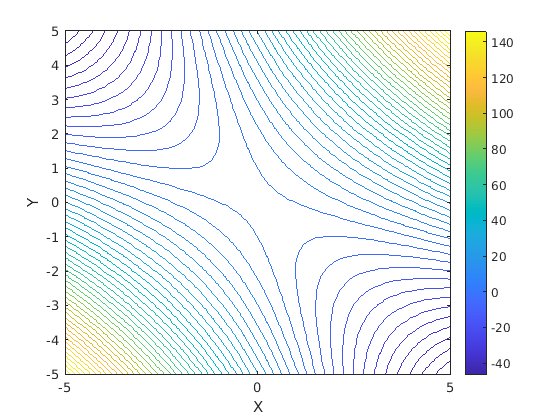
\includegraphics[width=\textwidth]{../Problem 1/contour_lines_2d.png}
		\caption{2D Plot}
		\label{fig:prob_1_contour_lines_2d}
	\end{subfigure}
	\begin{subfigure}{0.4\textwidth}
		\includesvg[width=\textwidth]{../Problem 1/contour_lines_3d.svg}
		\caption{3D Plot}
		\label{fig:prob_1_contour_lines_3d}
	\end{subfigure}
	\caption{Contour lines of $f(x,y)$ }
	\label{fig:prob_1_contour_lines}
\end{figure}

A general formula of a quadratic equation is $f(x,y) = ax^2 + 2bxy + cy^2$. Writing our formula in the previous form, we find that $a=1, \MathSpace b=2, \MathSpace c=1$.
Calculation of discriminant can help us calculate the location of function's local minimum/maximum.

\begin{equation}
\begin{gathered}
D =
\left[
\begin{array}{cc}
	f_{xx} & f_{xy} \\
	f_{yx} & f_{yy} \\
\end{array}
\right]
= f_{xx} f_{yy} - f^2_{xy} = 2 \times 2 - 4^2 = -12 < 0, \quad \text{όπου} \\
f_{xx} = \frac{\partial^2 f}{\partial x^2} = 2, \quad
f_{yy} = \frac{\partial^2 f}{\partial y^2} = 2, \quad
f_{xy} = \frac{\partial}{\partial y} \left( \frac{\partial f}{\partial x} \right) = 4
D = 2 \times 2 - 4^2 = -12 < 0.
\end{gathered}
\end{equation}

So, we only have to find the point where $\frac{\partial f}{\partial x}$ and $\frac{\partial f}{\partial y}$ are equal to $0$. Thus, this point will be a saddle point where gradients in each orthogonal direction are $0$, but this point is not either a local minimum or maximum.
Specifically:
\begin{equation}
\left\{
\begin{array}{c}
	\frac{\partial f}{\partial x} = 2x + 4y = 0 \\ 
	\frac{\partial f}{\partial y} = 4x + 2y = 0 \\
\end{array}
\right.
\Rightarrow
\left\{
\begin{array}{c}
	x = 0\\y=0\\
\end{array}
\right.
\end{equation}
Thus, the point $(x,y) = (0,0)$ is the saddle point mentioned before for the function given and this can be justified using the plotted contour lines.
	% !TeX spellcheck = en_US
\section{Problem 11}

Fuzzy logic is a type of logic that deals with vague, imprecise, or uncertain information. It is based on the concept of fuzzy sets, which are sets that can have any degree of membership between 0 and 1.  The value zero is used to represent complete non-membership, the value one is used to represent complete membership, and values in between are used to represent intermediate degrees of membership.This means that an element can be a member of a fuzzy set to some degree, rather than all or nothing.

The uniqueness of fuzzy logic is that fuzzy logic can handle imprecise and uncertain information,which makes it a valuable tool for dealing with real-life problems that are inherently vague or fuzzy. 

On this exercise, we are dealing with the linguistic variable \textit{Truth} with a possible membership set: 

\begin{center}
	\textit{T = {Absolutely false, Very false, False, Fairly true, True, Very true, Absolutely true}}
\end{center}

Based on that set we may define the membership function of truth as:
\begin{center}
	\textit{True(u) = u \hspace{3mm}  False(u) = 1-u}
\end{center}
for each $u \in [0, 1]$.

	






	% !TeX spellcheck = en_US
\section{Problem 12}

In order to evaluate the expression "\verb|not(A(x) OR B(x))|", we first have to take a look in how fuzzy logic is different with binary logic at the operation level.
In binary logic we have three basic operations: \verb*|AND(x,y)|, \verb*|OR(x,y)| and \verb*|NOT(x)|. But, in fuzzy logic, where a function can have a value in range of $\left[0...1\right]$, things are a bit different.
Operation \verb*|AND(x,y)| of binary is equivalent with \verb|MIN(x,y)| from the fuzzy logic, \verb*|OR(x,y)| with \verb*|MAX(x,y)| and \verb*|NOT(x)| with \verb|1-x|.

\begin{wrapfigure}{R}{0.5\textwidth}
	\centering
	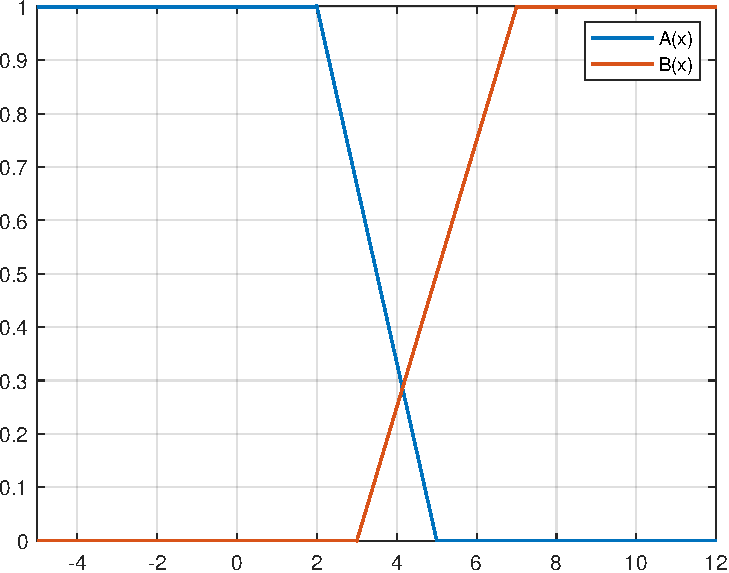
\includegraphics[width=0.4\textwidth]{../Problem 12/a_b_functions.pdf}
	\caption{Plot of A(x), B(x)}
	\label{fig:prob_12_a_b}
\end{wrapfigure}

We have to find the proper $x$ for which the previous expression has the greater value. Firstly, we will calculate the expression and then find the proper $x$.
To achieve this, we will have to break down our calculations in areas. 

Starting with $x \le 2$, $"A(x) \text{ AND } B(x)"$ is equal to $"\max\left(A(x), B(x)\right)" = 1$. So, using De Morgan's law, we have $\textit{max}\left(A(x), B(x)\right) = \textit{not}\left(A(x) \textit{ or } B(x)\right) = 0$.
The exact same result is obtained at $x \ge 7$.

Things are a bit different in $2 \le x \le 7$. Function $A(x)$ starts to fall while $B(x)$ starts to rise. The point where they cross is valuable for defining the expression needed and can be found by solving the equation 
\[
A(x) = B(x) \Leftrightarrow 1 - \frac{x-2}{3} = \frac{x-3}{4} \Rightarrow x = \frac{29}{7}
\]

So, for $2 \le x \le \frac{29}{7}$, $\textit{max}\left(A(x), B(x)\right) = 1 - \dfrac{x-2}{3} = A(x)$, because in this region $A(x)$ is above $B(x)$. Thus, $\textit{not}\left(A(x) \textit{ or } B(x)\right) = \dfrac{x-2}{3}$.

Using the same logic, we find out that for $\frac{29}{7} \le x \le 7$, $\textit{not}\left(A(x) \textit{ or } B(x)\right) = 1 - \dfrac{x-3}{4}$. 

Therefore, the expression $f(x) = \textit{not}\left(A(x) \textit{ or } B(x)\right)$ is summarized in the following:
\begin{equation}
	f(x) = \left\{
	\begin{array}{cc}
		0 & x \le 2, \\[3pt]
		\dfrac{x-2}{3} & 2 \le x \le \frac{29}{7}, \\[7pt]
		1 - \dfrac{x-3}{4} & \frac{29}{7} \le x \le 7, \\[3pt]
		0 & x \ge 7\\
	\end{array}
	\right.
\end{equation}
	
\end{document}